\section{Si}
\subsection*{Material ID: mp-cdhjp}
\textbf{Constante Dieléctrica ($\epsilon_{total}$):} 12.13 \\[0.5em]
\begin{table}[h!]
\centering
\begin{tabular}{lcc}
\toprule
\textbf{Métrica} & \textbf{Lámina (Plate)} & \textbf{Cilindros (Rod)} \\
\midrule
Bandgaps ($k_x$) & Ninguno & Ninguno \\
Resonancias ($k_x$) & 36 & 36 \\
\midrule
Bandgaps (Rotación) & Ninguno & Ninguno \\
Resonancias (Rotación) & 33 & 33 \\
\bottomrule
\end{tabular}
\end{table}
\begin{figure}[H]
\centering
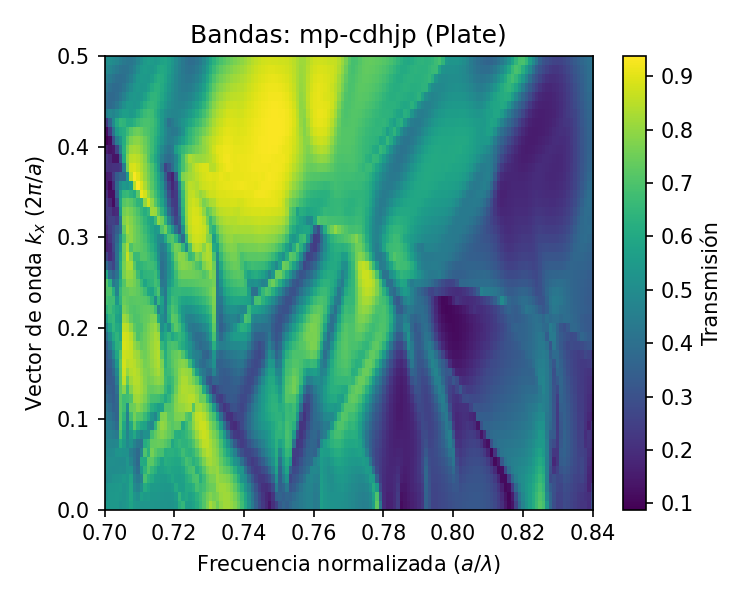
\includegraphics[width=0.48\textwidth]{figures/mp-cdhjp_plate.png}
\hfill
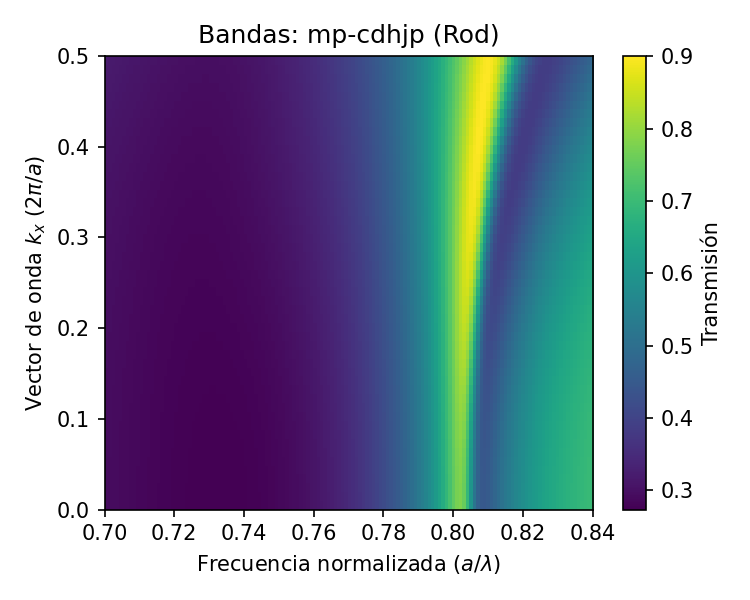
\includegraphics[width=0.48\textwidth]{figures/mp-cdhjp_rod.png}
\caption{Estructuras de bandas fotónicas ($k_x$) para mp-cdhjp. Izquierda: Lámina. Derecha: Cilindros.}
\end{figure}
\vspace{1em}
\begin{figure}[H]
\centering
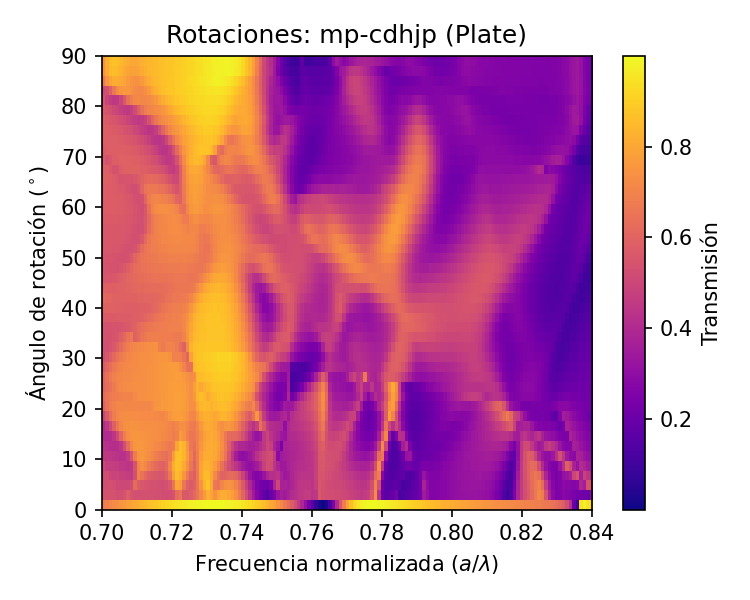
\includegraphics[width=0.48\textwidth]{figures/mp-cdhjp_plate_rangle.png}
\hfill
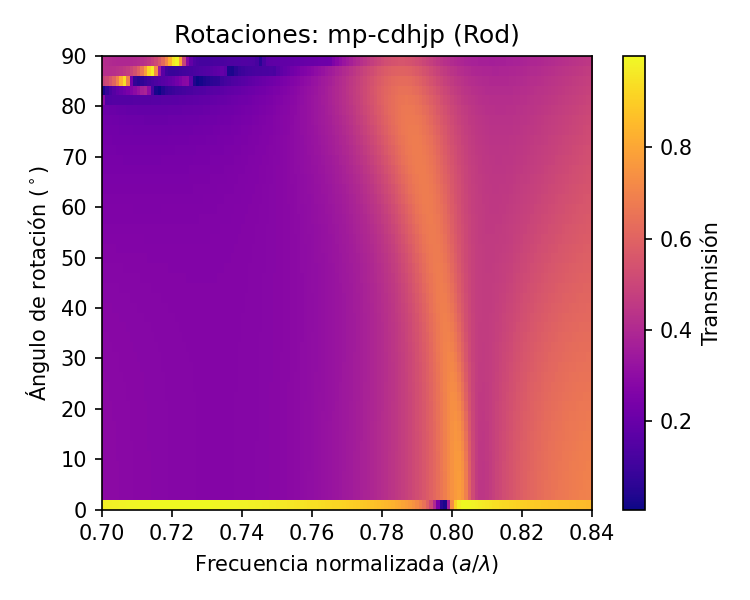
\includegraphics[width=0.48\textwidth]{figures/mp-cdhjp_rod_rangle.png}
\caption{Mapas de transmisión por rotación (twist) para mp-cdhjp. Izquierda: Lámina. Derecha: Cilindros.}
\end{figure}
\vspace{1em}
\hrule
\vspace{1em}
\subsection*{Material ID: mp-ft}
\textbf{Constante Dieléctrica ($\epsilon_{total}$):} 13.00 \\[0.5em]
\begin{table}[h!]
\centering
\begin{tabular}{lcc}
\toprule
\textbf{Métrica} & \textbf{Lámina (Plate)} & \textbf{Cilindros (Rod)} \\
\midrule
Bandgaps ($k_x$) & Ninguno & Ninguno \\
Resonancias ($k_x$) & 36 & 36 \\
\midrule
Bandgaps (Rotación) & Ninguno & Ninguno \\
Resonancias (Rotación) & 33 & 33 \\
\bottomrule
\end{tabular}
\end{table}
\begin{figure}[H]
\centering
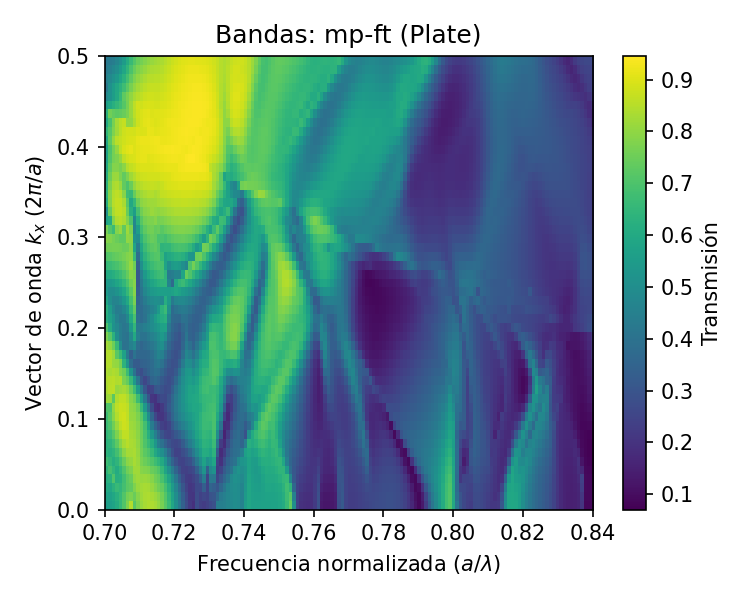
\includegraphics[width=0.48\textwidth]{figures/mp-ft_plate.png}
\hfill
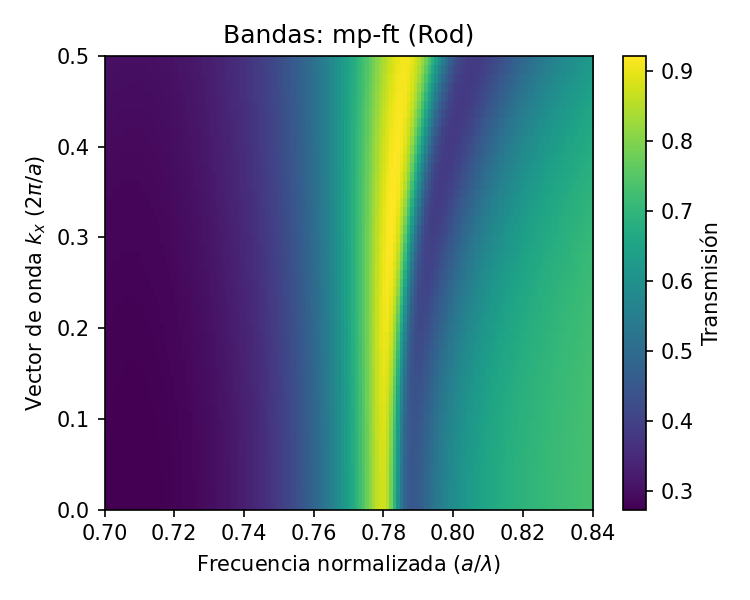
\includegraphics[width=0.48\textwidth]{figures/mp-ft_rod.png}
\caption{Estructuras de bandas fotónicas ($k_x$) para mp-ft. Izquierda: Lámina. Derecha: Cilindros.}
\end{figure}
\vspace{1em}
\begin{figure}[H]
\centering
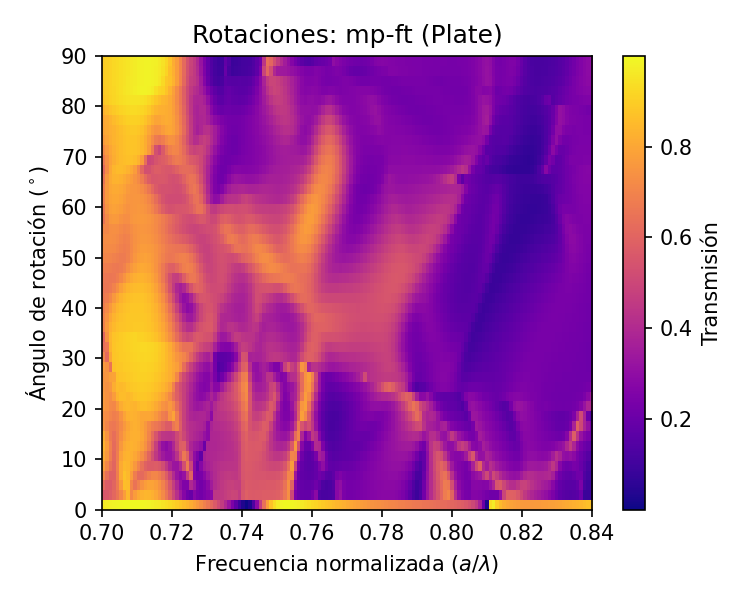
\includegraphics[width=0.48\textwidth]{figures/mp-ft_plate_rangle.png}
\hfill
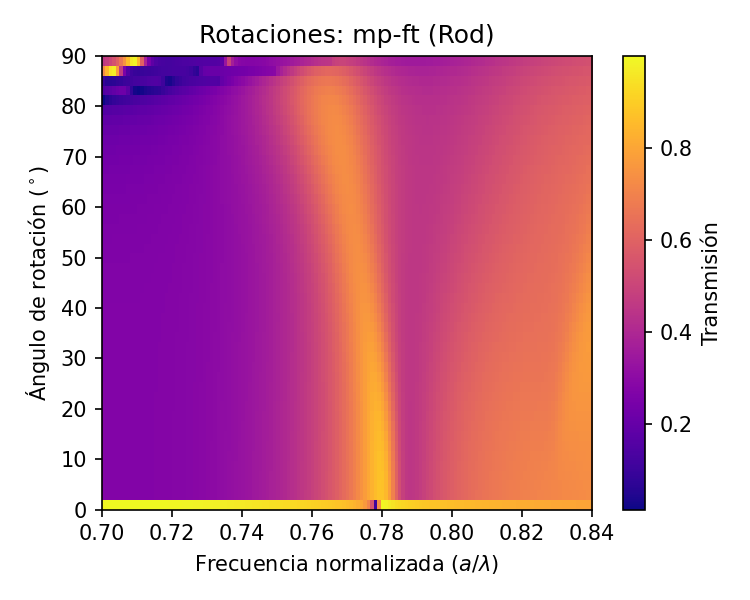
\includegraphics[width=0.48\textwidth]{figures/mp-ft_rod_rangle.png}
\caption{Mapas de transmisión por rotación (twist) para mp-ft. Izquierda: Lámina. Derecha: Cilindros.}
\end{figure}
\vspace{1em}
\hrule
\vspace{1em}
\subsection*{Material ID: mp-gj}
\textbf{Constante Dieléctrica ($\epsilon_{total}$):} 12.75 \\[0.5em]
\begin{table}[h!]
\centering
\begin{tabular}{lcc}
\toprule
\textbf{Métrica} & \textbf{Lámina (Plate)} & \textbf{Cilindros (Rod)} \\
\midrule
Bandgaps ($k_x$) & Ninguno & Ninguno \\
Resonancias ($k_x$) & 36 & 36 \\
\midrule
Bandgaps (Rotación) & Ninguno & Ninguno \\
Resonancias (Rotación) & 33 & 33 \\
\bottomrule
\end{tabular}
\end{table}
\begin{figure}[H]
\centering
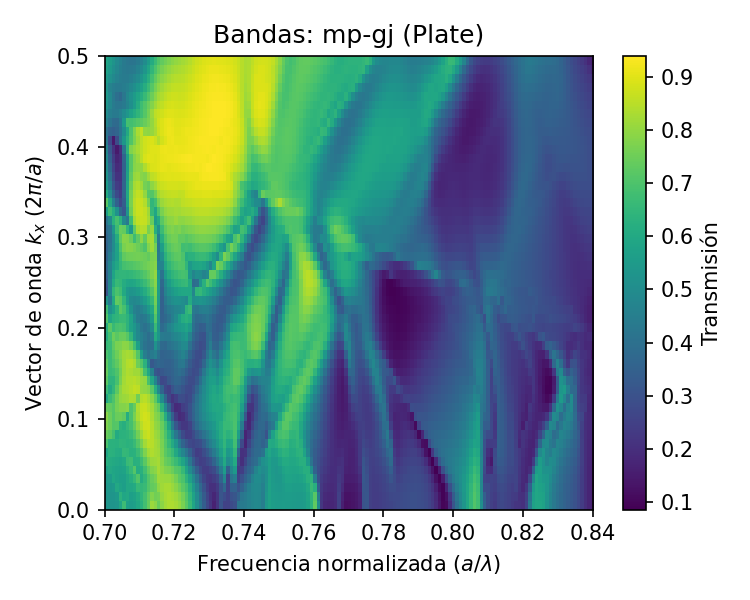
\includegraphics[width=0.48\textwidth]{figures/mp-gj_plate.png}
\hfill
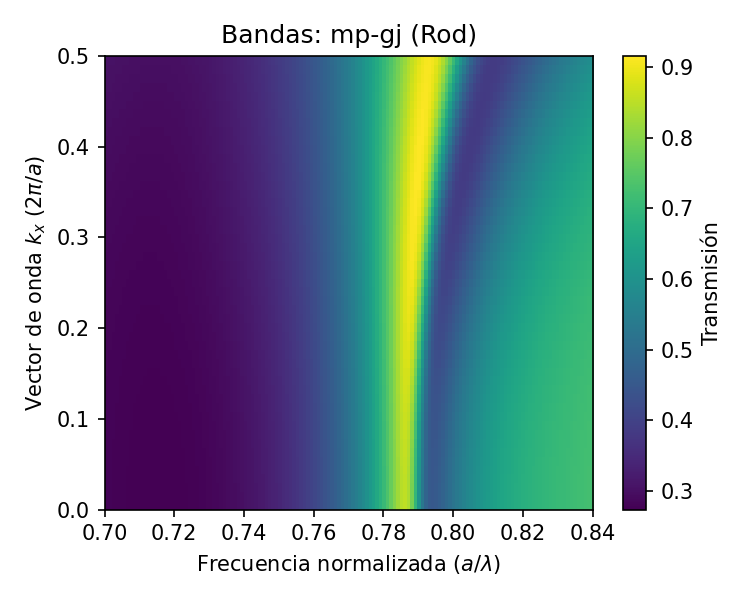
\includegraphics[width=0.48\textwidth]{figures/mp-gj_rod.png}
\caption{Estructuras de bandas fotónicas ($k_x$) para mp-gj. Izquierda: Lámina. Derecha: Cilindros.}
\end{figure}
\vspace{1em}
\begin{figure}[H]
\centering
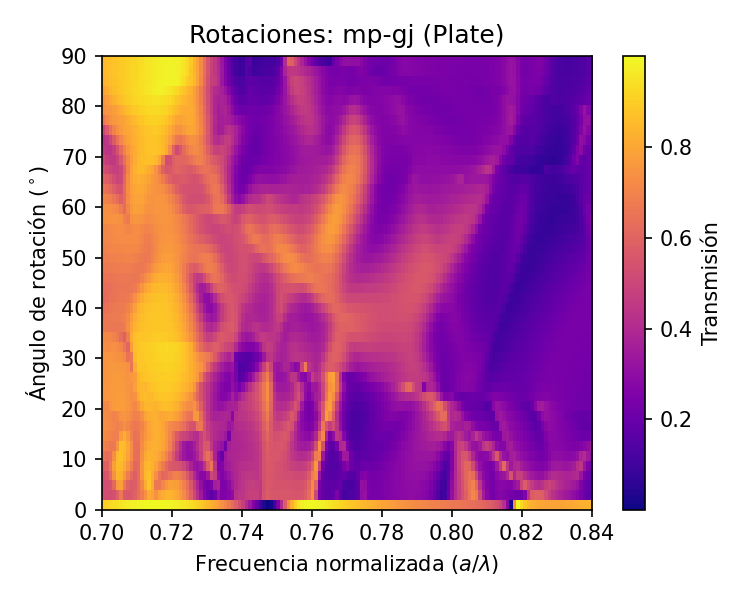
\includegraphics[width=0.48\textwidth]{figures/mp-gj_plate_rangle.png}
\hfill
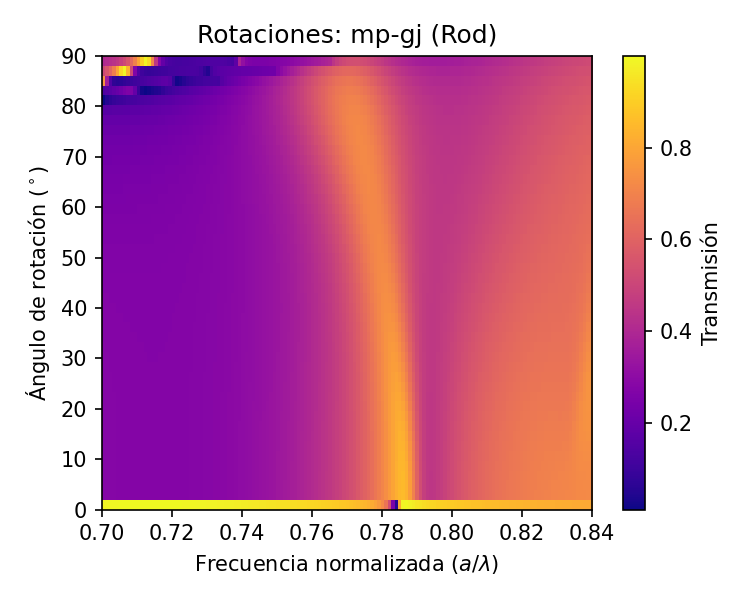
\includegraphics[width=0.48\textwidth]{figures/mp-gj_rod_rangle.png}
\caption{Mapas de transmisión por rotación (twist) para mp-gj. Izquierda: Lámina. Derecha: Cilindros.}
\end{figure}
\vspace{1em}
\hrule
\vspace{1em}
\clearpage